
\part{대기과학 실험}


%----------------------------------------------------------------------------------------
%	CHAPTER
%----------------------------------------------------------------------------------------

\chapter{기초 실험}

\section{빗방울의 낙하 속도}\index{빗방울의 낙하 속도}

Rain is the liquid form of precipitation on Earth. It is part of the hydrologic cycle that begins when water evaporates and forms clouds in the atmosphere. The water that forms these clouds is frozen and vaporized. Once enough water has evaporated, it is then released in the form of droplets of rain back to the surface of the Earth.

The average size of a raindrop is 6 millimeters in diameter, about the size of a housefly. Of course all raindrops vary in size due to the strength of a specific rainstorm, but this is considered a reasonable value of a typical raindrop. When a raindrop falls to the surface of the Earth, it is acted on by two main forces, gravity and drag. A stationary raindrop initially experiences an acceleration due to gravity of 9.8 m/s2, as would any falling body. As gravity increases the speed of the raindrop in its descent, drag retards the downward acceleration of the raindrop. Usually, air resistance that comes in contact with the water molecules as they fall causes the drag. The combination of these two forces causes a raindrop to reach a terminal velocity when the drag force is approximately equal to the weight of the raindrop. At this point, a raindrop experiences no further acceleration and therefore falls at a constant velocity.

The magnitude of the terminal velocity of an object is also affected by its orientation. A common misconception is the shape of the raindrop. It is often depicted as pointy and lopsided. However, research has found the shape of a raindrop to be rather spherical or slightly flattened on the bottom by airflow like a hamburger bun.

The terminal velocity of a 6-millimeter raindrop was found to be approximately 10 m/s. This value has been found to vary between 9 m/s and 13 m/s when measurements were taken on different days. The variance has been contributed to different air temperatures and pressures. In comparison, a human being falling to the surface of the Earth experiences a drastically larger terminal velocity of approximately 56 m/s.


How Fast Is Falling Rain? \cite{evan2007}

Let the physics begin. You might think: hey, wont’ the speed depend on how high the water started? Well, it would if air resistance on the water drop were not important. However, I suspect that the rain will fall at terminal velocity. Terminal velocity is the case when the air resistance on the object is equal to the gravitational force on the object. When this happens, the net force is zero (the zero vector) and the object falls at a constant speed.

Here is a diagram of a water drop at terminal speed.

Untitled 1
Since the air resistance force depends on the speed of the object (but the gravitational force does not), there is one speed for which these two forces add up to the zero vector. Near the surface of the Earth, the magnitude of the gravitational force can be modeled as:

La te xi t 1 4

Where g is the local gravitational field (not the acceleration due to gravity – that is a non-good name for it). And what about the air resistance? It can probably be modeled as:

La te xi t 1 5

Where:

ρ is the density of air (about 1.2 kg/m3).
A is the cross-sectional area of the object. If the object was a sphere, this area would be the area of a circle.
C is the drag coefficient. This depends on the shape of the object. A cone and a flat circle will have the same A, but different drag coefficients.
v is the magnitude of the velocity of the object with respect to the air.
It won’t matter for this case too much, but the direction of the air resistance force is in the opposite direction to the velocity.
At terminal velocity, the magnitudes of these two forces will be equal. I can write that as:

La te xi t 1 6

Now, what about the mass (m)? Let me assume that it is made of water (like most rain) and is spherical (even though that is not likely – it would probably be “rain drop shaped”). If I call the density of water ρw and the radius of the drop r, then the mass would be:

La te xi t 1 7

Putting this into the “weight = air resistance” expression above as well as an expression for the cross-sectional area in terms of r, I get:

La te xi t 1 8

The cool thing here is that the terminal speed of the water drop depends on the size (radius). Larger drops will have a larger terminal velocity. So, could you just make a water melon sized water drop? No. Why not? Because at some point, the force from the air on the drop is going to break the water drop apart. The surface tension holding the drop together just won’t be enough to maintain its drop status.

Then how big can it get? I have no idea. Oh, and then there is the problem of real drop instead of spherical drops. Let me look at that first. Wikipedia lists the coefficient of drag for a smooth sphere as 0.1. A rain drop should be less than this – but how much less? Well, a rain drop would take some of the water to form some sort of tail. This would decrease the cross sectional area as well as decrease the drag coefficient. I am not sure how to calculate the volume of a non-spherical rain drop, so for now I will just use a spherical drop with a drag coefficient of 0.08. I know that is wrong, but it will give me an idea about the terminal speed.

Now, how big should it be? How about I don’t decide. Instead I will plot the terminal speed for a range of rain drop sizes. Let me look at drops from 0.5 mm to 5 mm. Here is that plot.

Raindrop.png

Well, the original question asked about the speeds in units of miles per hour. Here is the same plot but with different units.

Raindrop 2.png

Based on my estimations, 17 mph would be on the low end – but possible. It could be likely that I grossly overestimated the size of a raindrop.

Homework: Yes, there is homework. If the rain drop has a radius of 0.5 mm, from how high would it have to drop to get pretty close to the terminal velocity?


UPDATE


As usual, I rush into things without exploring things in more depth. My assumption of a raindrop shaped raindrop appears to be bogus. Who would have guessed that? Anyway, here are some very useful links from commenters (Jens and Charles) and a large thanks to them.

A German kid’s video showing the shape of a raindrop (I think).
A nice summary of findings for falling rain drops.
Terminal Velocity of Rain Drops Aloft – paper from the Journal of Applied Meteorology (pdf)
Here is another link from @swansontea: Bad Rain: Raindrops are not tear drop shaped.

%----------------------------------------------------------------------------------------
%	CHAPTER 
%----------------------------------------------------------------------------------------

\chapter{대기의 안정도와 단열선도}

\section{단열선도}
1930년대부터 고층기상관측이 실시되면서 대기를 입체적으로 파악하게 되었다. 고층기상관
측 자료를 신속하게 정리·분석하여 한 관측 지점의 연직방향 열역학적 특성을 파악하는데 단
열선도가 이용되고 있다. 단열선도는 복잡한 수식으로 계산해야 하는 기상 현상이나 기상요소
를 간단히 구할 수 있도록 고안된 도표이다. 단열선도에는 여러 종류가 있으나 어느 것이나 건
조 단열선, 습윤 단열선, 포화 혼합비선, 등온선, 등압선의 5선이 그려져 있다. 온도와 기압이
기울어져 Skew T-log P diagram라는 명명된 단열선도<그림 Ⅲ-18>이 가장 많이 쓰이고 있다.

\begin{figure}[h]
	\centering
	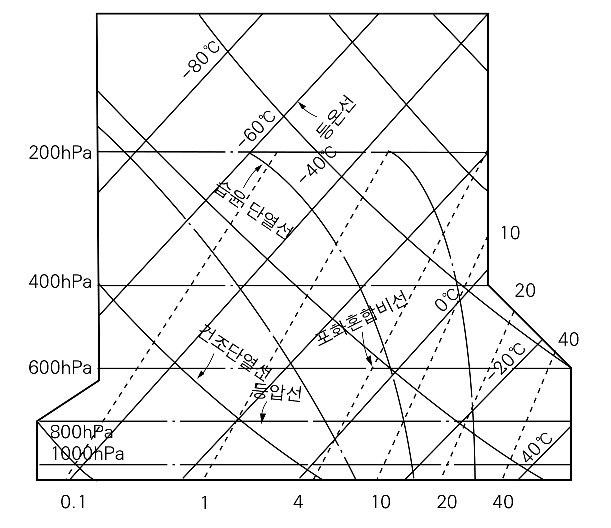
\includegraphics[width=0.8\linewidth]{skewT-logP-1}
	\caption{단열선도의 구성 선들}
	\label{fig:skewt-logp}
\end{figure}

단열선도에서 구할 수 있는 기상요소들은 다음과 같다.
① 혼합비 : 건조공기 1 kg 속에 혼합된 수증기의 질량(g)으로 Skew T-log P diagram에서
는 알고자 하는 고도의 이슬점 온도를 지나는 포화혼합비선의 값을 읽으면 된다.
② 상대습도 : R.H(%) = 실제 혼합비/ 포화 혼합비  ×100이므로 Skew T-log P diagram에서는
R.H(%)= 이슬점 온도에 해당하는 혼합비/ 기온에 해당하는 혼합비 
이 된다.
③ 상승응결고도(LCL, Lifting Condensation Level) : 온도점에서 건조 단열선을 따라 올라간
선과 이슬점에서 포화 혼합비선을 따라 올라간 선이 만나는 점의 고도이다.
④ 대류응결고도(CCL, Convection Condensation Level) : 상승응결고도에서 포화 혼합비선을
따라 올라간 선과 기온 곡선이 만나는 점의 고도이다


\section{사용 실례}\index{단열선도 사용 실례}

예를 들어 기압이 1000 hPa, 기온 3 ℃, 상대습도 70%인 공기덩어리(A점)가 위로 상승한다
고 가정하자. 기온 3 ℃에서의 포화혼합비를 그림에서 구하면 5 g이므로 이 공기의 혼합비는
그 70%인 3.5 g이다. 이 값은 공기 중의 수증기가 응결되어 줄어 들거나 또는 외부로부터 공
급되지 않는 한 변하지 않는다. 이 공기덩어리가 상층으로 올라가면 단열적으로 변화하므로
단열선도의 건조 단열선을 따라 기압이 내려간다. 그리고 925 hPa 부근에서 3.5 g의 혼합비선
과 만난다. 이것은 이 공기덩어리의 상대습도가 점차 증가하여 여기서 100% 즉, 포화에 도달
된다는 것을 의미한다. 따라서 그 이상의 고도로 올라가면 공기덩어리 중의 수증기가 응결하
면서 변화하게 되므로 기온이 습윤 단열선을 따라 변해간다. 수증기가 응결하기 시작하는 이
고도를 응결고도 또는 구름이 생성되는 높이이므로 운저고도(雲底高度), 운고라 한다. 이 예에
서 응결고도는 925 hPa 고도이며 대략 지상 750 m 정도가 된다.

\begin{figure}[h]
	\centering
	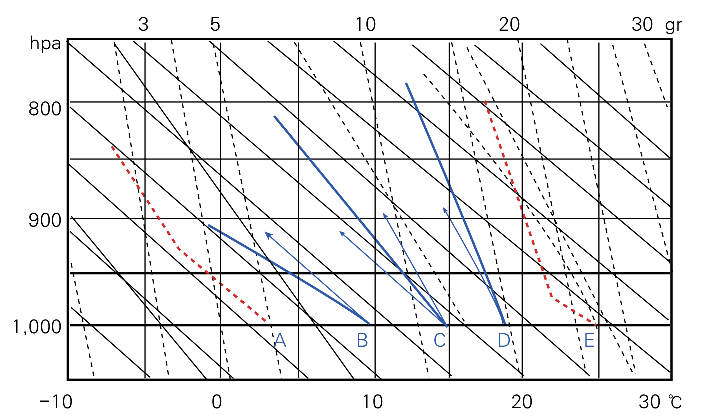
\includegraphics[width=0.8\linewidth]{skewT-logP-2}
	\caption{단열선도 이용 실례}
	\label{fig:skewt-logp-1}
\end{figure}


\section{대기 안정도 분석}\index{단열선도를 이용한 대기 안정도 분석}

단열선도를 이용하면 대기층의 안정 상태를 쉽게 파악할 수 있다. 고층관측 결과를 단열선
도에 기입했을 때 대기의 온도가 <그림 Ⅲ-19>의 굵은 선 B와 같이 변하였다고 하자. 지상의
공기덩어리를 상층으로 가지고 올라갔을 때의 상황을 조사해 보면, 그림에서 파선과 같이 되
므로 이 공기덩어리의 기온은 주위 공기의 기온보다 높아져 밀도가 작아지므로 부력을 받아
계속 상승하려 한다. 그래서 이런 상태의 대기성층을 불안정이라 한다. 이런 때는 대류가 일
어난다. 여기서 알 수 있는 것처럼 대기의 실제 기온감률이 100 m당 1 ℃ 이상이면 그 기층은
불안정하다는 것을 알 수 있으며, 특히 이 경우를 절대 불안정이라 한다.
대기의 온도 변화가 <그림 Ⅲ-19>에서 굵은 선 C와 같았다고 할 경우에는, 그 기층의 공기
가 포화되지 않고 건조하다면 건조 단열선을 따라 변하므로 상공으로 올라가면서 밀도가 본래
의 대기 밀도보다 커지므로 안정하게 된다. 그런데 공기가 포화되어 있으면 습윤 단열선을 따
라 변하므로 상공에 올라가 주위 공기보다 기온이 높아져 불안정해진다. 이상으로 보면 수증
기 함유량에 따라 안정하기도 하고 불안정하기도 한다. 이것을 조건부 불안정이라 한다.
<그림 Ⅲ-19>에서 D와 같은 경우에는 공기가 건조한 경우나 습윤한 경우에 관계 없이 위로
올라간 공기덩어리는 주위 공기보다 기온이 낮아 안정적이다. 이것을 기온감률로 표현하면 실
제 기온감률이 습윤단열변화 할 때보다 작은 경우로서 대기의 기온감률이 100 m당 0.5 ℃ 미
만인 경우이다. 이를 절대 안정이라 한다.
만일 실제 기온의 고도변화가 100 m 당 1 ℃라면 공기덩어리가 건조단열 변화하면서 상승
해도 주위와의 기온차가 생기지 않는다. 또 기온의 고도변화가 습윤 단열선을 따르는 상태에
서는 포화된 공기덩어리는 상승해도 주위와의 기온차가 없다. 즉, 안정도 불안정도 아닌 중립
상태가 된다.
<그림 Ⅲ-19>의 E의 경우는 파선을 따라 변화한다. 따라서 이 경우 885hPa이하에서는 안정
이나 그 이상 끌어올리면 주위보다 기온이 높아져 불안정이 된다. 즉 요란이 작으면 안정 상태
를 유지하지만, 요란이 크면 불안정하게 된다. 이러한 상태를 잠재 불안정이라 한다.


%------------------------------------------------



\begin{definition}[단열선도를 이용한 대기 분석]
	
	
	열선도 중에서 가장 널리 이용되고 있는 Skew T-log P diagram 상에 실제 관측 자료를 표시하여 여러 가지 기상현상을 구해보고, 이를 통해 대기를 입체적으로 분석해 보자.
	
	1. 다음 표는 고층 기상 관측 자료이다.
	
	
	\begin{tabular}{c|c|c|c|c|c}
		\hline 
		기압(hPa) & 기온(℃) & 이슬점  온도 & 혼합비(g/kg) & 포화혼합비 & 상대습도(\%) \\ \hline 
		1000 & 25 & 14 &	 &  &  \\ 
		\hline 
		900 & 18 & 6 &  &  &  \\ 
		\hline 
		800 & 8 & -1 &  &  &  \\ 
		\hline 
		700 & 3 & -12  &  &  &  \\ 
		\hline 
		600 & 0 & -10 &  &  &  \\ 
		\hline 
		500 & -13 & -151 &  &  &  \\ 
		\hline 
		400 & -16 &-40	&  &  &  \\ 
		\hline 
	\end{tabular} 
	
	
\end{align}
\end{definition}

%------------------------------------------------
